\documentclass[12pt]{article}

\usepackage[margin=0.74in]{geometry}
\usepackage{iftex}
\ifPDFTeX
  \usepackage[T1]{fontenc}
  \usepackage{newtxtext,newtxmath}
\else
  \usepackage{fontspec}
  \setmainfont{Times New Roman}
\fi
\usepackage{graphicx}
\usepackage{booktabs}
\usepackage{tabularx}
\usepackage{array}
\usepackage{float}
\usepackage{caption}
\usepackage{subcaption}
\usepackage{titlesec}
\usepackage{enumitem}
\usepackage{titling}
\usepackage{indentfirst}
\usepackage{hyperref}
\usepackage{xcolor}

\hypersetup{
  colorlinks=true,
  linkcolor=black,
  urlcolor=blue,
  citecolor=black
}

\graphicspath{{plot/fig/}}
\setlength{\parindent}{0.5cm}
\setlength{\parskip}{0pt}
\setlength{\textfloatsep}{3pt plus 1pt minus 1pt}
\setlength{\floatsep}{3pt plus 1pt minus 1pt}
\setlength{\intextsep}{3pt plus 1pt minus 1pt}
\setlength{\abovecaptionskip}{2pt}
\setlength{\belowcaptionskip}{0pt}
\renewcommand{\arraystretch}{1.0}
\captionsetup{skip=2pt}
\setlist[itemize]{topsep=2pt,itemsep=1pt,parsep=0pt,partopsep=0pt,leftmargin=1.2em}
\titleformat{\section}{\normalfont\bfseries\fontsize{12pt}{14pt}\selectfont}{\thesection.}{0.5em}{}
\titleformat{\subsection}{\normalfont\bfseries\fontsize{12pt}{14pt}\selectfont}{\thesubsection.}{0.5em}{}
\titleformat{\subsubsection}{\normalfont\itshape\fontsize{12pt}{14pt}\selectfont}{\thesubsubsection.}{0.5em}{}
\titlespacing*{\section}{0pt}{8pt plus 1pt minus 1pt}{4pt}
\titlespacing*{\subsection}{0pt}{6pt plus 1pt minus 1pt}{3pt}
\titlespacing*{\subsubsection}{0pt}{4pt plus 1pt minus 1pt}{2pt}
\setlength{\droptitle}{-2.2em}
\pretitle{\begin{center}\bfseries\fontsize{12pt}{14pt}\selectfont}
\posttitle{\par\end{center}\vspace{\baselineskip}}
\preauthor{\begin{center}\fontsize{12pt}{14pt}\selectfont}
\postauthor{\par\end{center}\vspace{0pt}}
\predate{\begin{center}\fontsize{12pt}{14pt}\selectfont}
\postdate{\par\end{center}\vspace{-1.4em}}
\linespread{0.95}

\title{Census Income Take-Home Report}
\author{Xinchun Ran}
\date{\today}

\begin{document}
\maketitle

\section{Executive Summary}

This submission solves two connected tasks on the Census Income dataset:
weighted binary classification of whether a record belongs to the income group
above \$50K, and interpretable customer segmentation for marketing activation.
The final workflow explicitly addresses class imbalance, preserves structural
categories such as \texttt{?} and \texttt{Not in universe}, and uses survey
weights for evaluation and segment profiling.

The classification comparison now includes not only ROC and PR curves, but also
threshold policy, calibration, score separation, and bootstrap uncertainty. On
the held-out test split, XGBoost attains the highest weighted ROC-AUC at 0.9555,
while LightGBM delivers the best weighted PR-AUC at 0.6845 and the best
thresholded weighted F1 among the deployed operating points at 0.6137. LightGBM
is also the best calibrated model, with weighted expected calibration error
0.0029 versus 0.0036 for XGBoost and 0.1629 for FT-Transformer. For that reason,
LightGBM remains the recommended production classifier.

The segmentation section now compares the pure unsupervised baseline
(\texttt{V1}) and the classifier-informed extension (\texttt{V2}) in the same
family of figures.
Version 1 yields the better cluster-quality trade-off for the main submission,
with $k=5$, silhouette 0.381, and composite score 1.722. Version 2 is more
stable, with pairwise agreement 0.975, and it splits the high-income population
into several finer premium-oriented subsegments. The recommended client-facing
story is therefore: use LightGBM for propensity scoring, keep Version 1 as the
main segmentation result, and use Version 2 as an advanced activation layer when
finer premium targeting is needed.

\section{Problem Framing And Data Constraints}

The take-home requires a report that is both technically credible and usable by
a business client. The dataset contains 40 demographic and employment variables,
one survey-weight column, and one binary income label. Four constraints are most
important:

\begin{itemize}
\item \textbf{Class imbalance.} The positive class is much smaller than the
negative class, so PR-AUC, weighted log loss, threshold tuning, and ranking
quality matter more than raw accuracy.
\item \textbf{Structural missingness.} Tokens such as \texttt{?} and
\texttt{Not in universe} carry signal and should not be dropped or blindly
imputed away.
\item \textbf{Mixed-type, high-cardinality tabular features.} This motivates
model-specific handling across CatBoost, XGBoost, LightGBM, and FT-Transformer.
\item \textbf{Survey weights.} The \texttt{weight} column is excluded from the
feature space, but used in training where supported, in all reported evaluation
metrics, and in segment summaries.
\end{itemize}

The final splits contain 119,713 training rows, 39,905 validation rows, and
39,905 test rows. A persistent row identifier is used throughout to prevent
leakage and to keep segmentation artifacts joinable.

\subsection{Exploratory Data Analysis}

Figure~\ref{fig:eda-overview} gives one compact data-exploration checkpoint. The
positive class is small in both row count and weighted population share, the
survey weights have a broad distribution, and the raw age / weeks-worked
differences already suggest why income prediction is learnable in this dataset.

\begin{figure}[!t]
\centering
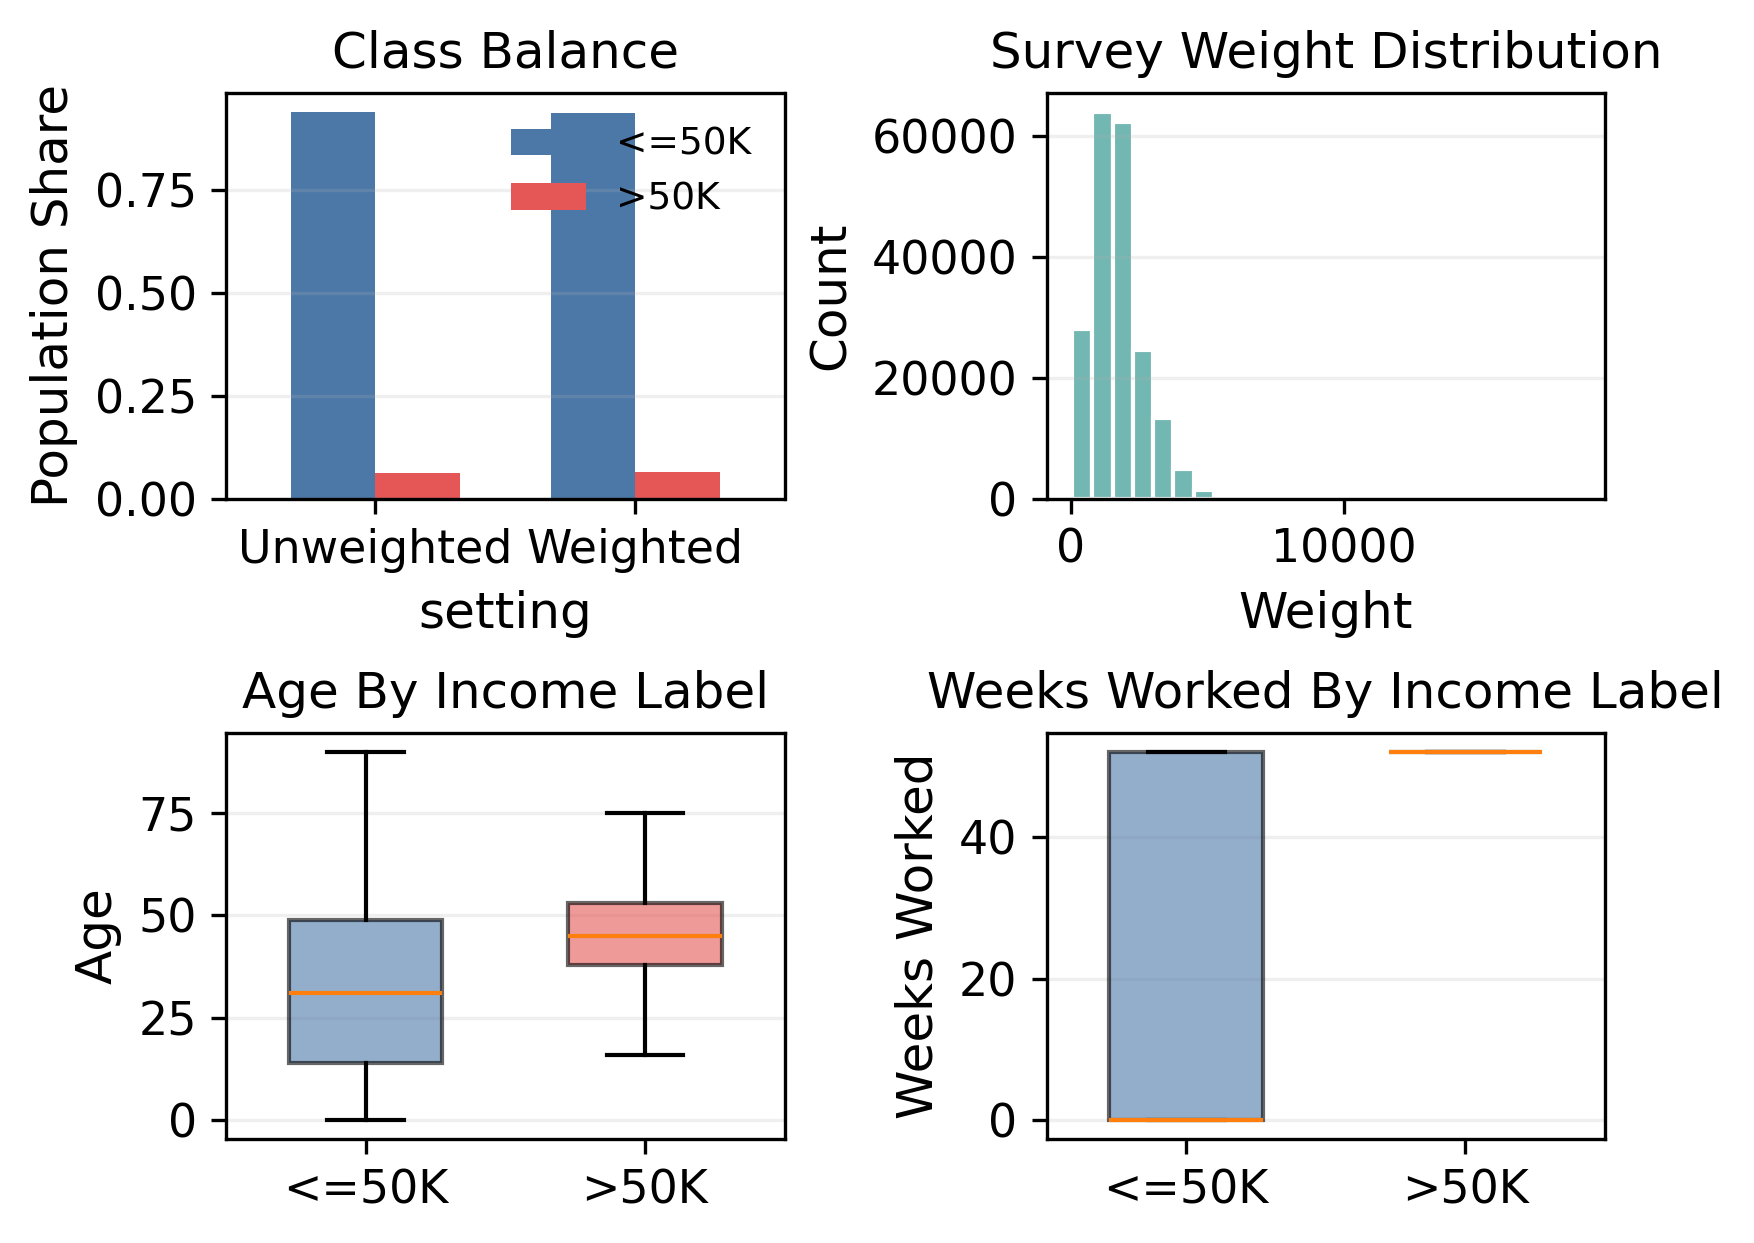
\includegraphics[width=0.72\linewidth]{eda_overview.png}
\caption{Exploratory data analysis overview: class balance, weight distribution,
age by income label, and weeks worked by income label.}
\label{fig:eda-overview}
\end{figure}

\section{Modeling Approach}

\subsection{Classification}

The classification stack compares CatBoost, XGBoost, LightGBM, and
FT-Transformer. Exported prediction artifacts keep a logit-first design:

\begin{center}
\texttt{logit} $\rightarrow$ \texttt{probability = sigmoid(logit)} $\rightarrow$
\texttt{predicted\_label}
\end{center}

This is important because the same score supports ranking, calibration, and
business threshold changes without rerunning the full model.

Preprocessing and training decisions are aligned with the take-home brief.
Structural categories such as \texttt{?} and \texttt{Not in universe} are
preserved as categories rather than collapsed into ordinary missingness. The
pipeline uses model-specific handling for mixed-type inputs, persistent row
identifiers for fixed train/validation/test splits, and sample weights in
training where the estimator supports them. All final model comparisons are
reported on the hold-out test split, while the operating threshold is tuned on
validation only. This separation is important because the deployed decision rule
should be selected before looking at final test performance.

\subsection{Segmentation}

Two segmentation pipelines are retained:

\begin{itemize}
\item \textbf{Version 1:} pure raw-feature unsupervised segmentation using the
engineered demographic and employment feature set only.
\item \textbf{Version 2:} classifier-informed segmentation that augments the
same feature set with the model-derived income propensity score.
\end{itemize}

Version 1 is built from a curated demographic and employment feature subset that
includes numeric variables such as age, weeks worked, veterans benefits, and
number of persons worked for employer; engineered binary asset indicators for
capital gains, losses, and dividends; and banded variables such as age band and
weeks-worked band. Numeric columns are median-imputed and scaled, categorical
columns are most-frequent-imputed and one-hot encoded, and the resulting feature
space is used as the input to MiniBatchKMeans. Version 2 reuses exactly this V1
feature space and adds the model-derived income propensity score as an auxiliary
signal, which shifts the clustering geometry toward finer premium-oriented
splits. The true income label is still excluded, so V2 is classifier-informed
but not supervised clustering with respect to the target label.

Cluster count is not chosen by one metric alone. The pipeline searches
$k \in \{3,4,5,6,7,8\}$ and ranks candidates with the internal score
`silhouette + 1/(1+DB) + log(1+CH)/10 - 0.5 * 1(min cluster share < 1\%)`.
This rewards separation, penalizes overlap, adds a tempered compactness term,
and subtracts a fixed penalty for tiny clusters. Stability is then used as a
post-selection robustness check rather than a direct ingredient in the
composite score, which keeps the $k$ selection rule transparent.

\section{Classification Results}

\subsection{Cross-Validation And Hold-Out Performance}

Table~\ref{tab:cv-results} summarizes mean weighted cross-validation
performance. LightGBM and XGBoost clearly outperform CatBoost and
FT-Transformer, with nearly identical ROC behavior and a small PR/log-loss edge
for LightGBM.

\begin{table}[!htbp]
\centering
\small
\caption{Mean weighted cross-validation metrics.}
\label{tab:cv-results}
\begin{tabular}{lccc}
\toprule
Model & ROC-AUC & PR-AUC & Weighted Log Loss \\
\midrule
CatBoost & 0.943 & 0.627 & 0.127 \\
XGBoost & 0.952 & 0.682 & 0.116 \\
LightGBM & 0.952 & 0.685 & 0.115 \\
FT-Transformer & 0.937 & 0.563 & 0.339 \\
\bottomrule
\end{tabular}
\end{table}

Table~\ref{tab:test-results} uses the exported test predictions. XGBoost gives
the best ROC-AUC, but LightGBM remains the preferred final model because it
improves PR-AUC and operating F1 while also achieving the lowest weighted log
loss. This matters more for an imbalanced targeting problem than a marginal ROC
gain alone.

\begin{table}[!htbp]
\centering
\small
\caption{Held-out weighted test metrics. Operating F1 uses each model's deployed threshold
(0.38 for LightGBM, 0.50 for XGBoost, 0.82 for FT-Transformer).}
\label{tab:test-results}
\begin{tabular}{lcccc}
\toprule
Model & ROC-AUC & PR-AUC & Weighted Log Loss & Operating F1 \\
\midrule
XGBoost & 0.9555 & 0.6799 & 0.1141 & 0.5746 \\
LightGBM & 0.9549 & 0.6845 & 0.1139 & 0.6137 \\
FT-Transformer & 0.9413 & 0.5775 & 0.3115 & 0.5482 \\
\bottomrule
\end{tabular}
\end{table}

\begin{figure}[!htbp]
\centering
\begin{subfigure}[t]{0.48\linewidth}
\centering
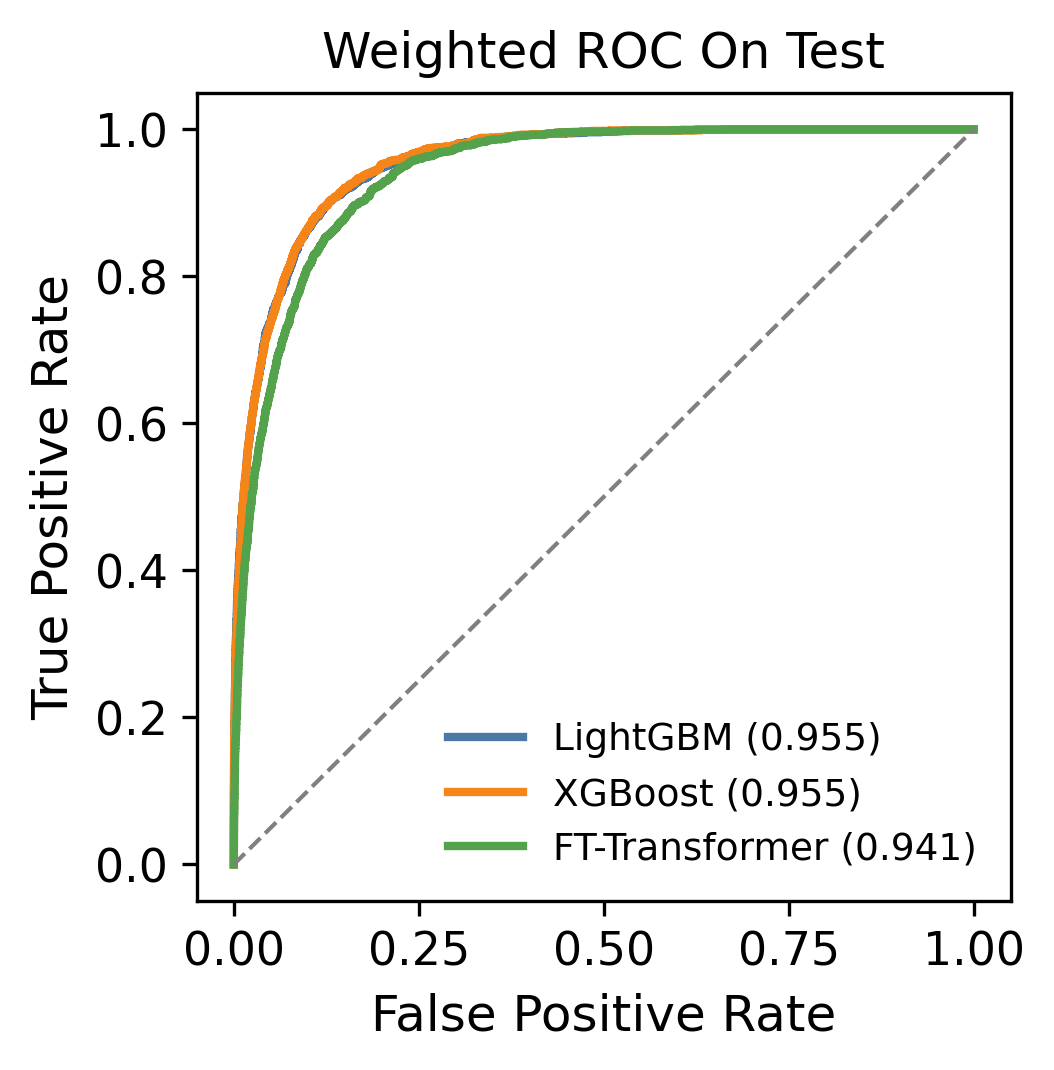
\includegraphics[width=\linewidth]{classification_roc_test.png}
\caption{Weighted ROC on test.}
\label{fig:roc}
\end{subfigure}
\hfill
\begin{subfigure}[t]{0.48\linewidth}
\centering
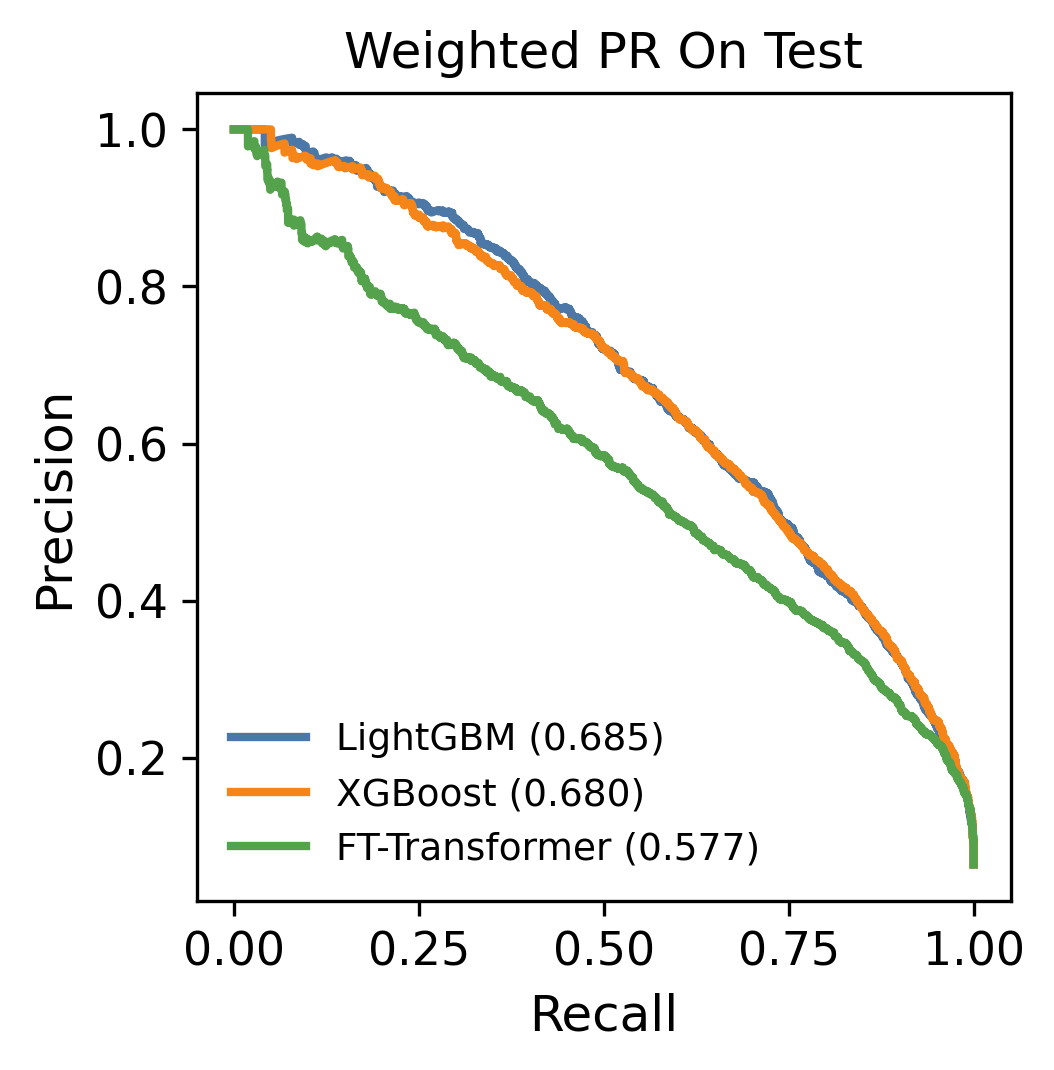
\includegraphics[width=\linewidth]{classification_pr_test.png}
\caption{Weighted PR on test.}
\label{fig:pr}
\end{subfigure}
\caption{Discrimination quality of the three exported classifiers.}
\label{fig:roc-pr-pair}
\end{figure}

Figures~\ref{fig:roc-pr-pair} and~\ref{fig:policy-calibration} show why the
model-selection story is stronger than a single metric table. XGBoost and
LightGBM are almost tied on ROC, but LightGBM keeps slightly better precision in
the actionable recall region and is materially better calibrated. The
FT-Transformer baseline is not only weaker in discrimination but also much less
well calibrated.

\subsection{Why Boosted Trees Won Here}

I do not interpret the LightGBM result as a generic statement that deep tabular
models are weak. I interpret it as a dataset-regime judgment. This problem is a
mixed-type census table with strong categorical structure, moderate feature
engineering leverage, and clear benefit from well-calibrated ranking scores; in
that regime, boosted trees are often the safer and stronger choice. The evidence
here is consistent across metrics: LightGBM and XGBoost beat FT-Transformer on
PR-AUC, weighted log loss, deployed operating F1, and calibration. FT-Transformer
was retained deliberately as a neural tabular benchmark to test whether learned
representations could outperform gradient boosting on this feature regime, but
it did not. In production I would therefore treat FT-Transformer as an
informative benchmark, not as a competitive deployment candidate for this
dataset.

\subsection{Threshold Policy, Calibration, And Uncertainty}

The validation threshold sweep for LightGBM converts the threshold from a magic
number into a policy decision. Figure~\ref{fig:policy-calibration} shows that
weighted F1 peaks around 0.38, exactly matching the saved threshold artifact.
At that point, the targeted weighted population share is about 5.8\% on the
validation split. This is a useful operating point for selective outreach:
precision remains high while recall is still meaningfully above the level that a
0.50 threshold would produce.

The same figure also reports calibration. LightGBM has weighted ECE 0.0029 and
XGBoost has weighted ECE 0.0036, indicating that both tree ensembles are
well-behaved probability models. FT-Transformer has ECE 0.1629 and therefore is
not reliable enough to use as a direct calibrated confidence score without
substantial post-processing.

\subsection{Business Decision Framework}

The preferred operating objective is \textbf{selective outreach for premium
margin efficiency}, not maximal audience reach. That is why precision matters
more than raw recall at deployment time: a marketing client typically pays for
every premium impression, contact, or offer, so false positives create direct
budget waste and channel fatigue. At the selected threshold of 0.38, the model
targets about 5.8\% of weighted population on validation, which is operationally
consistent with a focused premium campaign rather than a broad awareness push.
The ranking view tells the same story on test: the top 5\% scored weighted
population reaches 68.8\% observed positive rate, or about 10.8x lift over the
6.4\% weighted base rate; the top 10\% still reaches 48.5\%, or about 7.6x
lift. I recommend treating this threshold as a policy choice, not merely a
validation artifact. It is appropriate when the client has limited high-value
offer inventory and wants stronger expected value per contact rather than
maximum coverage.

\begin{figure}[!htbp]
\centering
\begin{subfigure}[t]{0.48\linewidth}
\centering
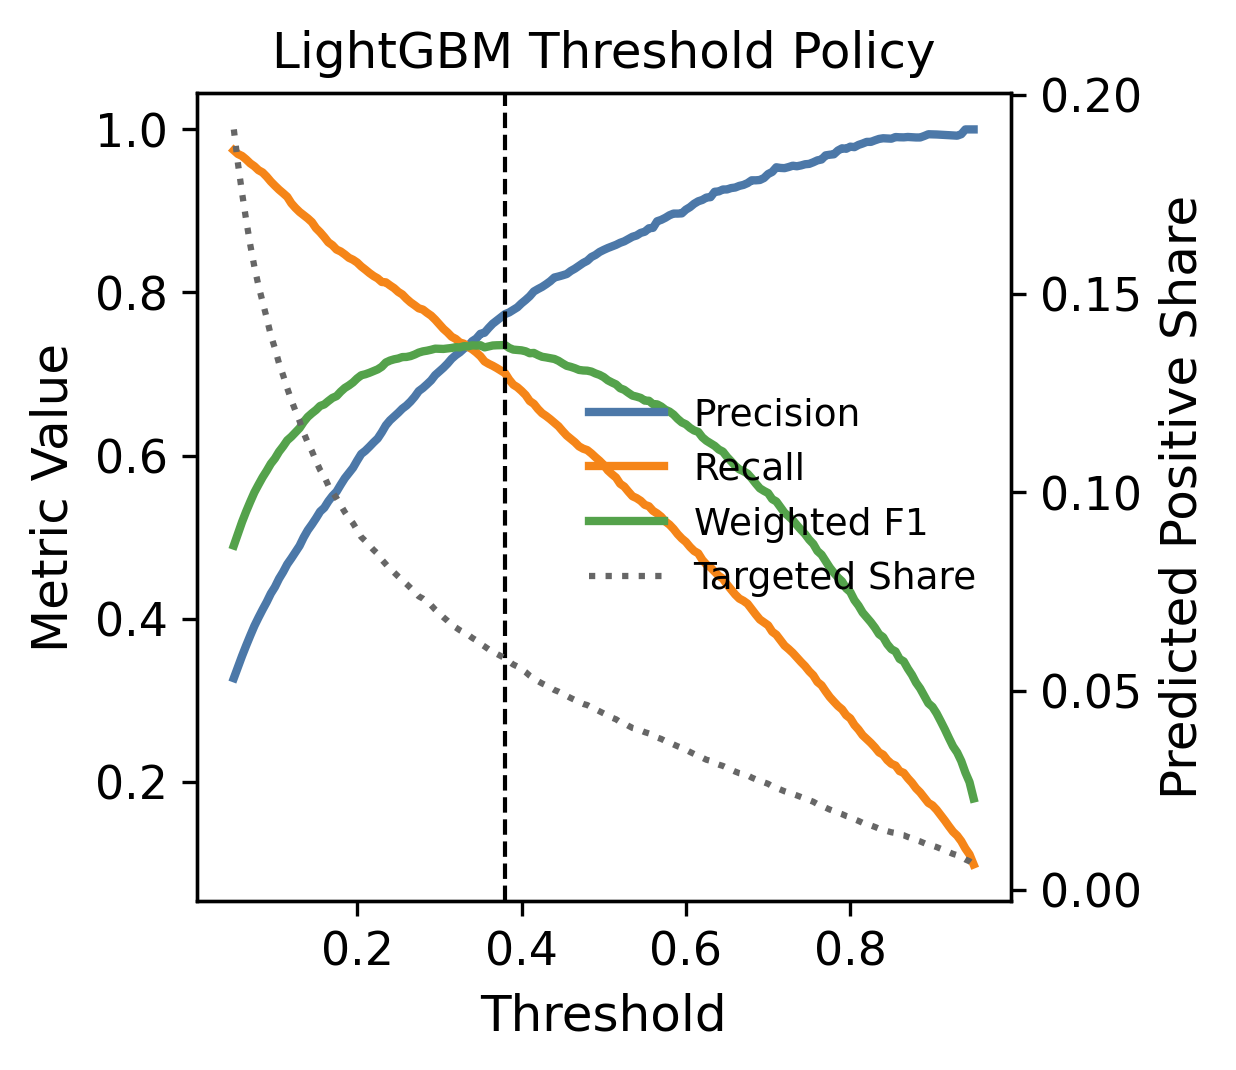
\includegraphics[width=\linewidth]{lightgbm_threshold_sweep_valid.png}
\caption{Validation threshold policy for LightGBM.}
\label{fig:threshold}
\end{subfigure}
\hfill
\begin{subfigure}[t]{0.48\linewidth}
\centering
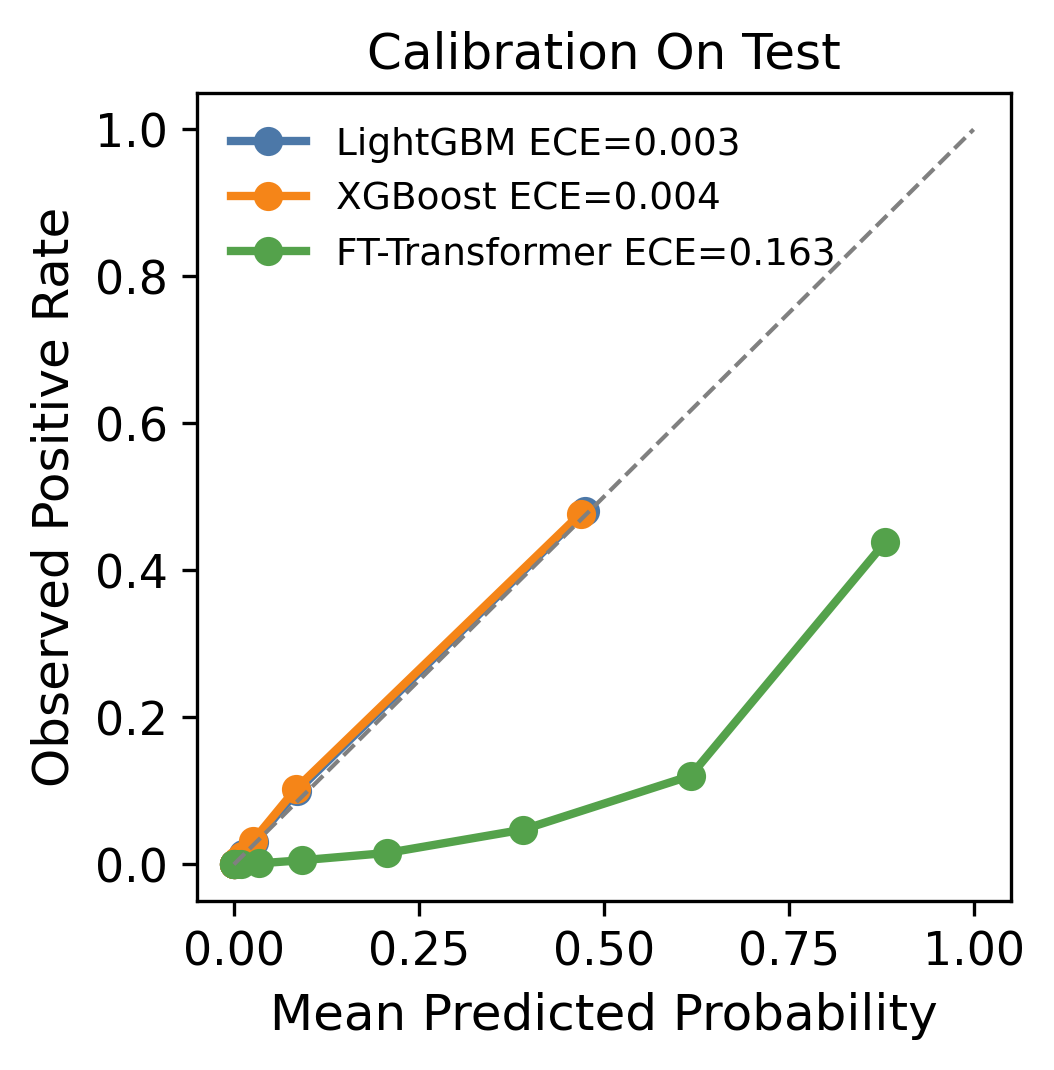
\includegraphics[width=\linewidth]{classification_calibration_compare.png}
\caption{Weighted calibration comparison on test.}
\label{fig:calibration}
\end{subfigure}
\caption{Threshold choice and score calibration.}
\label{fig:policy-calibration}
\end{figure}

Figure~\ref{fig:distribution-uncertainty} adds two more pieces of evidence. The
score distribution plot shows that the LightGBM probability mass for the positive
class is shifted clearly to the right, though with some overlap around the
decision region as expected in census income data. The three-model performance
comparison with bootstrap 95\% intervals shows that the ranking among models is
not a fluke: LightGBM and XGBoost overlap strongly on ROC, but LightGBM has the
strongest thresholded F1 profile among the deployed operating thresholds.

\begin{figure}[!htbp]
\centering
\begin{subfigure}[t]{0.48\linewidth}
\centering
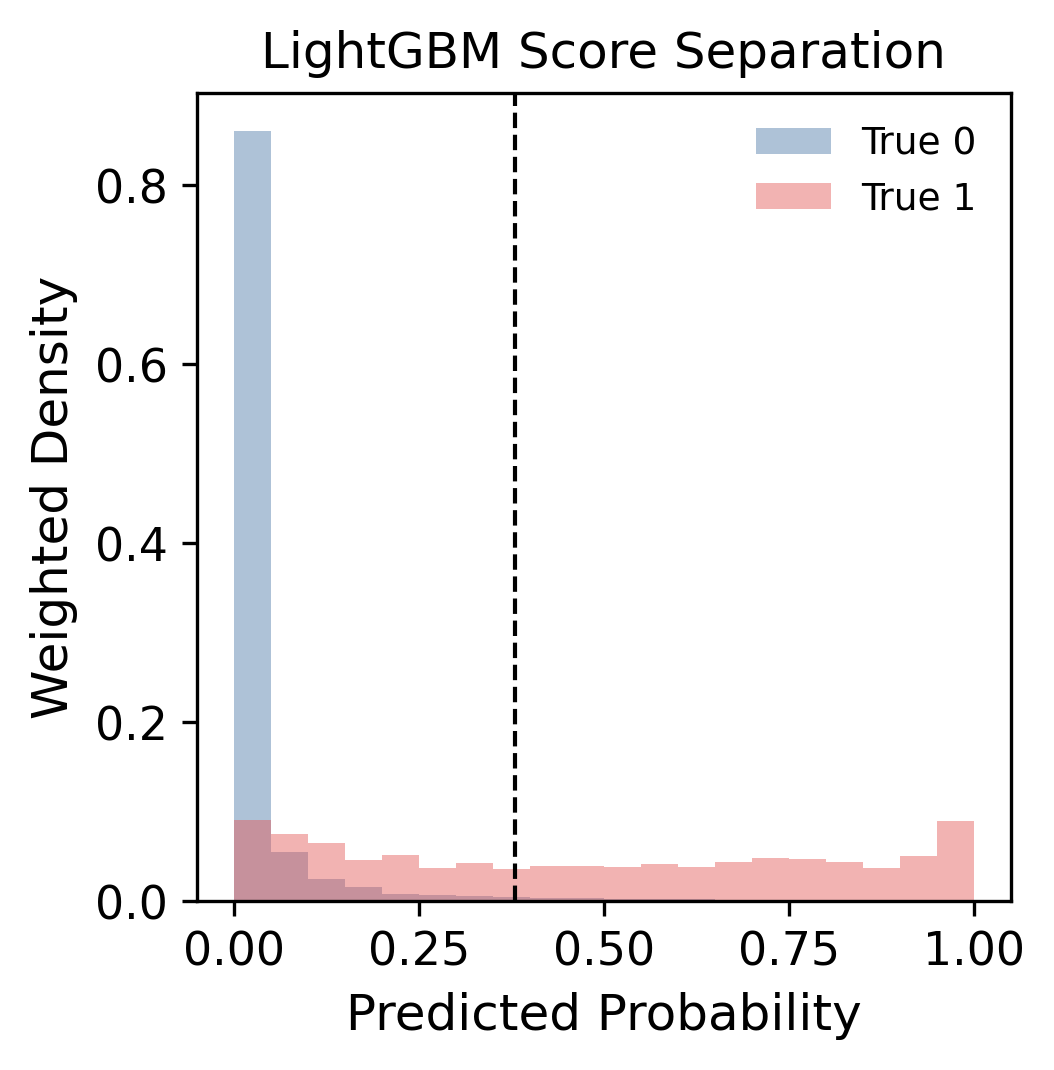
\includegraphics[width=\linewidth]{lightgbm_score_distribution.png}
\caption{LightGBM score separation by true class.}
\label{fig:score-dist}
\end{subfigure}
\hfill
\begin{subfigure}[t]{0.48\linewidth}
\centering
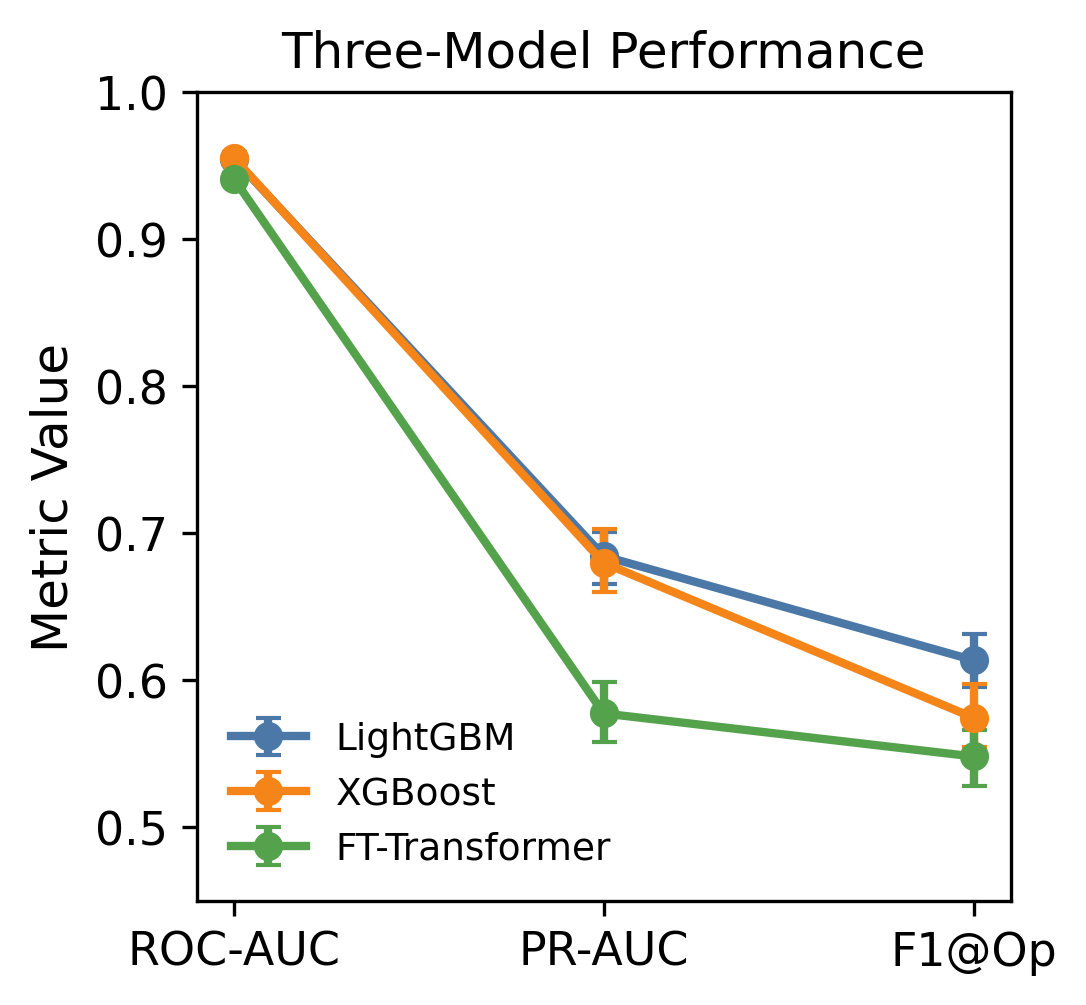
\includegraphics[width=\linewidth]{classification_metric_comparison.png}
\caption{Three-model performance with bootstrap CI.}
\label{fig:metric-compare}
\end{subfigure}
\caption{Confidence structure and uncertainty-aware model comparison.}
\label{fig:distribution-uncertainty}
\end{figure}

The bootstrap intervals are narrow enough to support a stable conclusion. For
LightGBM, the 95\% bootstrap interval is approximately [0.9515, 0.9585] for
ROC-AUC, [0.6658, 0.7009] for PR-AUC, and [0.5956, 0.6317] for operating F1.
Those intervals support the decision to treat the model as production-ready.

\begin{figure}[!htbp]
\centering
\begin{subfigure}[t]{0.48\linewidth}
\centering
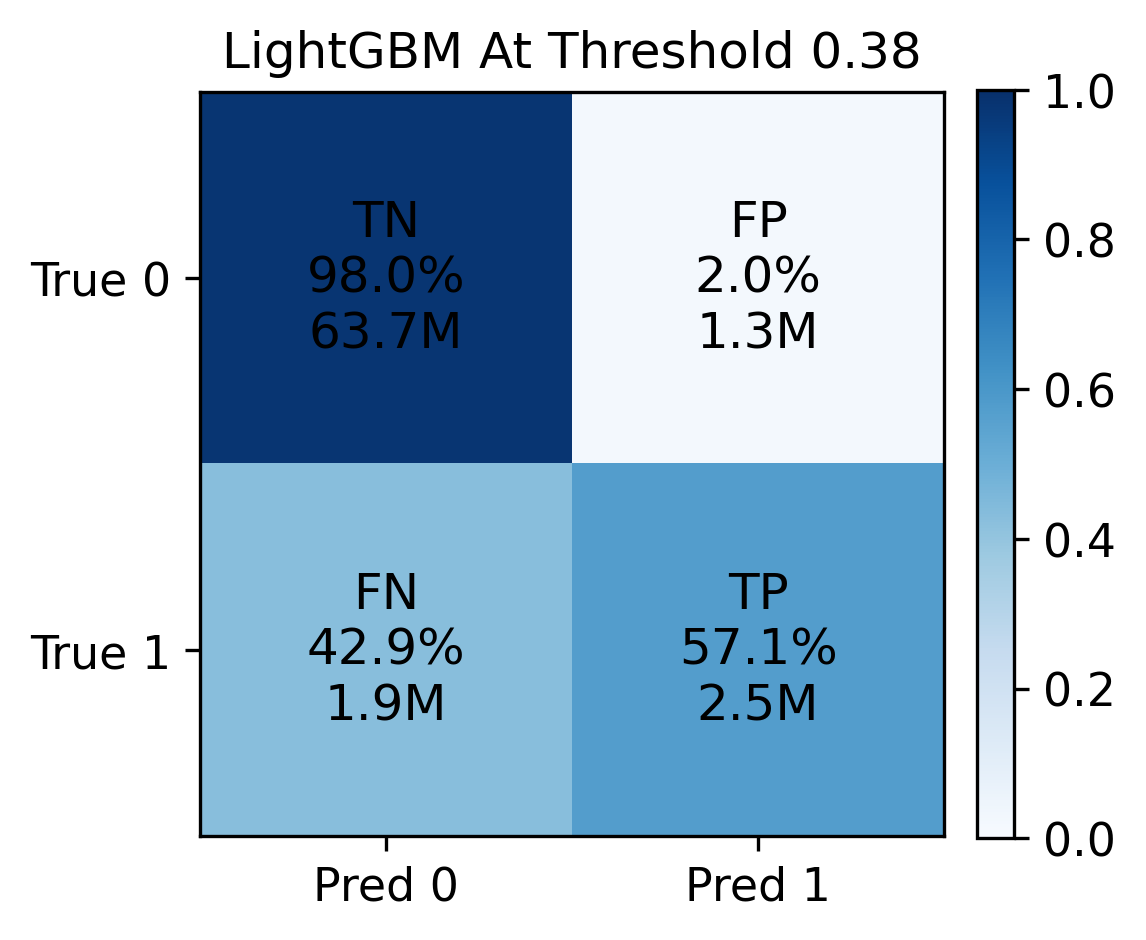
\includegraphics[width=\linewidth]{lightgbm_confusion_matrix_test.png}
\caption{Weighted confusion matrix at threshold 0.38.}
\label{fig:cm}
\end{subfigure}
\hfill
\begin{subfigure}[t]{0.48\linewidth}
\centering
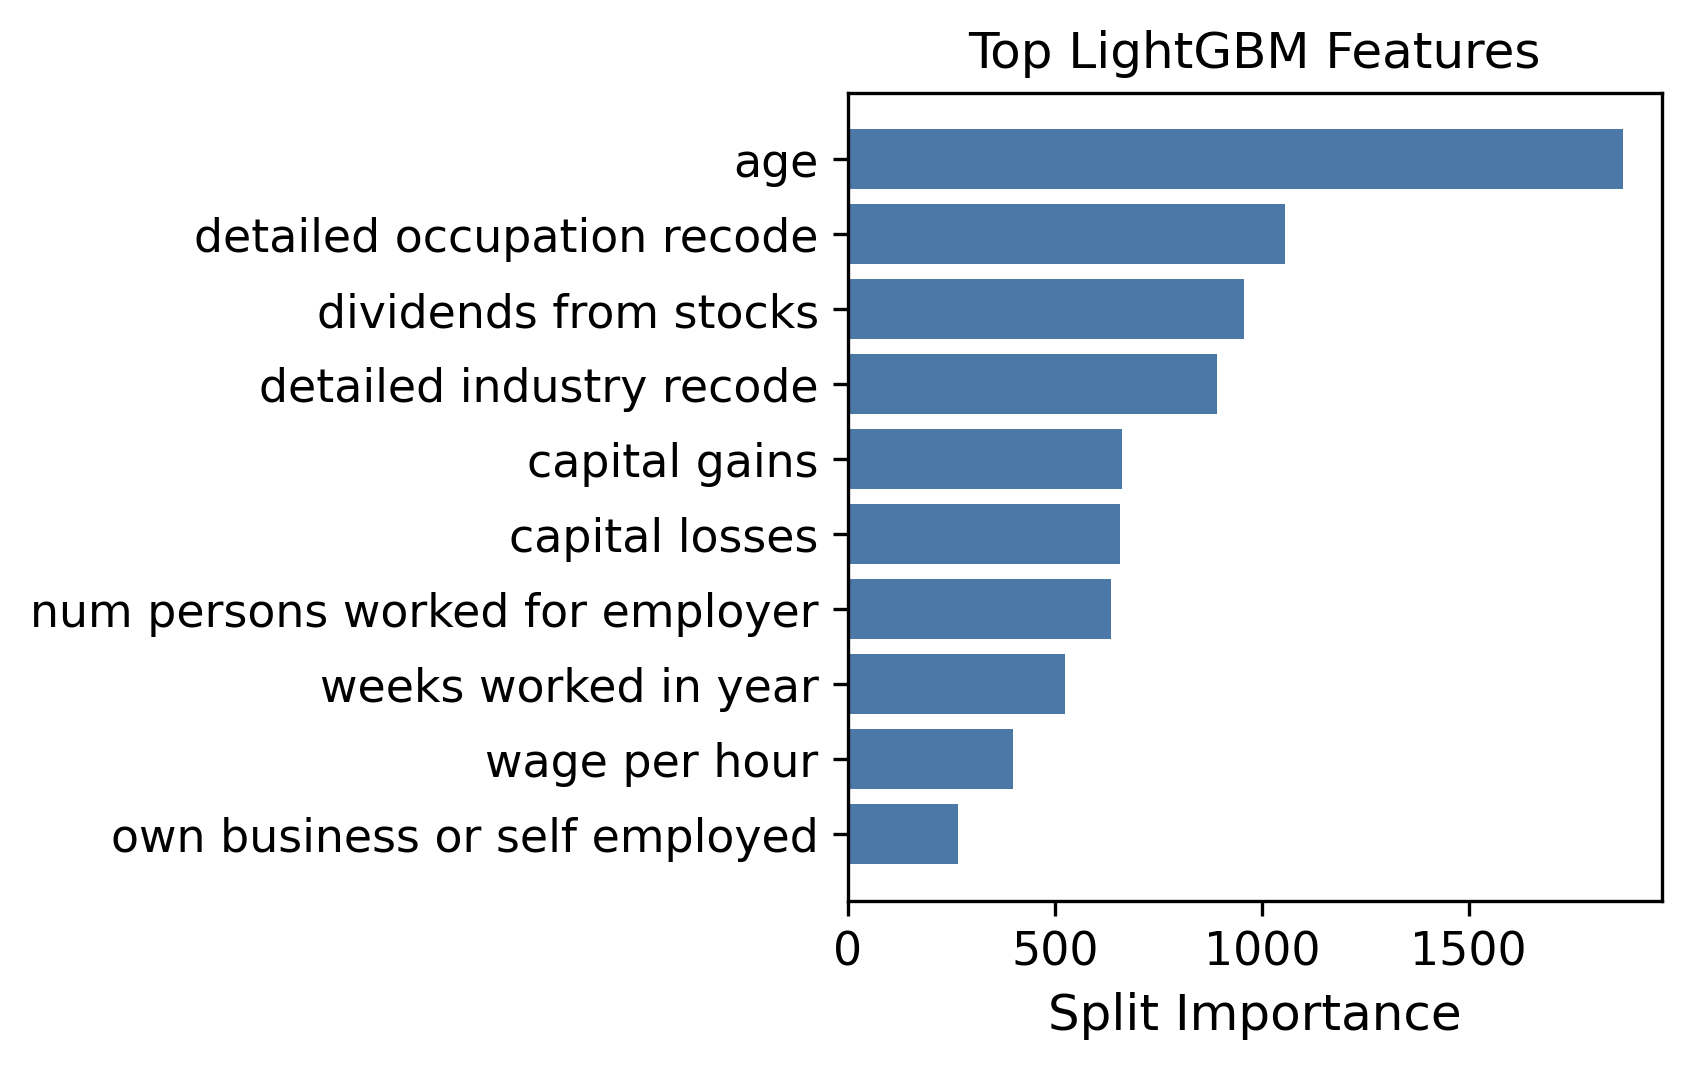
\includegraphics[width=\linewidth]{lightgbm_feature_importance.png}
\caption{Top LightGBM split-based importances.}
\label{fig:importance}
\end{subfigure}
\caption{Operating behavior and model explanation for the selected classifier.}
\label{fig:ops-explain}
\end{figure}

Figure~\ref{fig:ops-explain} closes the classification argument. The confusion
matrix shows that the tuned threshold still controls false positives while
substantially recovering positives. The feature-importance summary matches domain
intuition: age, occupation, dividends, industry, capital gains and losses, and
weeks worked all remain strong predictors of higher income.
I treat this split-based importance plot as directional evidence rather than a
final causal explanation. If I were extending the project further, the next
explanation upgrade would be permutation importance or a compact SHAP summary to
test whether the same feature ranking remains stable under a stronger
model-agnostic lens.

\section{Segmentation Results}

\subsection{Version 1 Vs Version 2}

The segmentation analysis is now organized as an explicit comparison between the
pure unsupervised baseline and the classifier-informed extension. This makes the
trade-off transparent: Version 1 is cleaner and more interpretable as a primary
submission artifact, while Version 2 is useful for finer-grained actionability.

\begin{figure}[!htbp]
\centering
\begin{subfigure}[t]{0.48\linewidth}
\centering
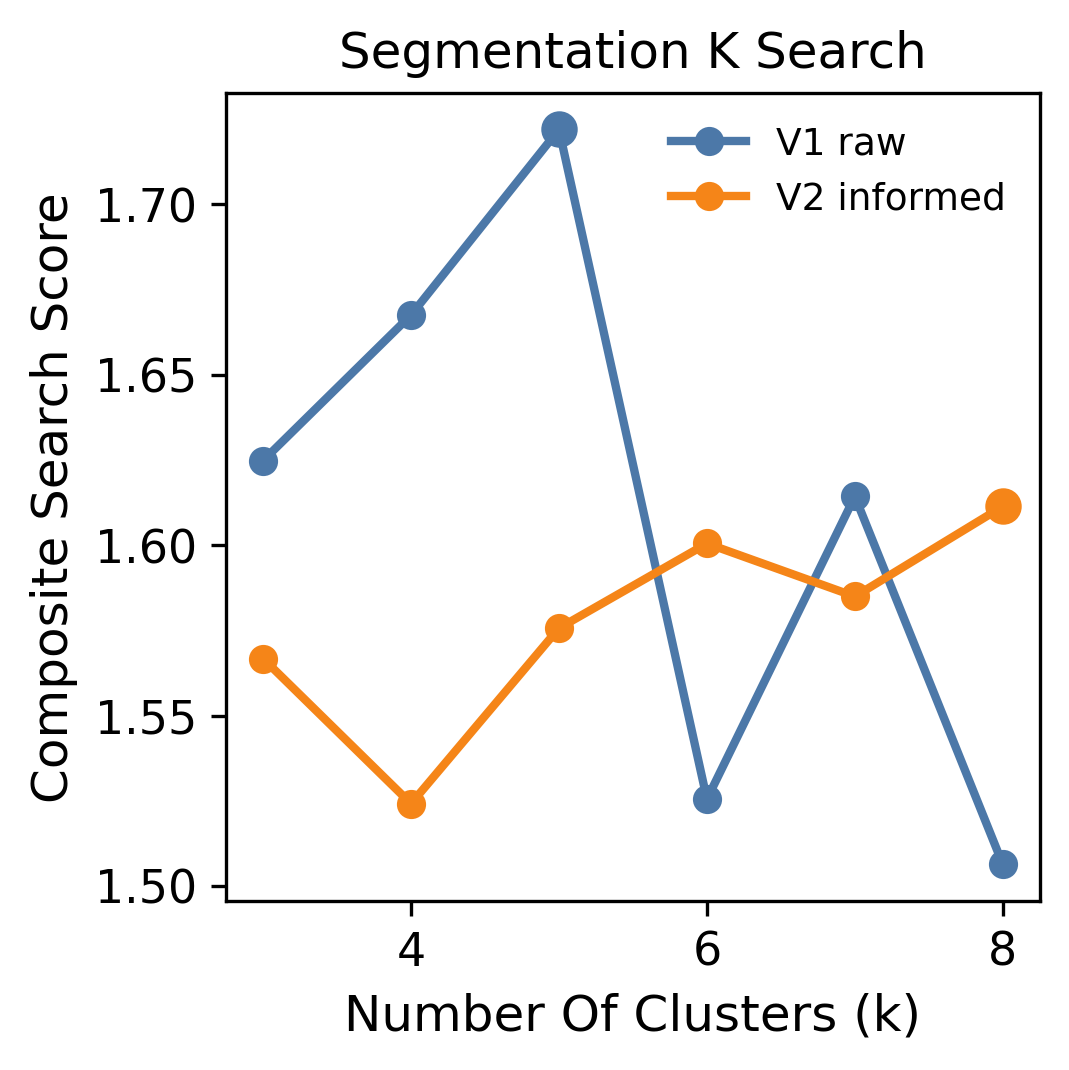
\includegraphics[width=\linewidth]{segmentation_k_search.png}
\caption{K-search score for V1 and V2.}
\label{fig:ksearch}
\end{subfigure}
\hfill
\begin{subfigure}[t]{0.48\linewidth}
\centering
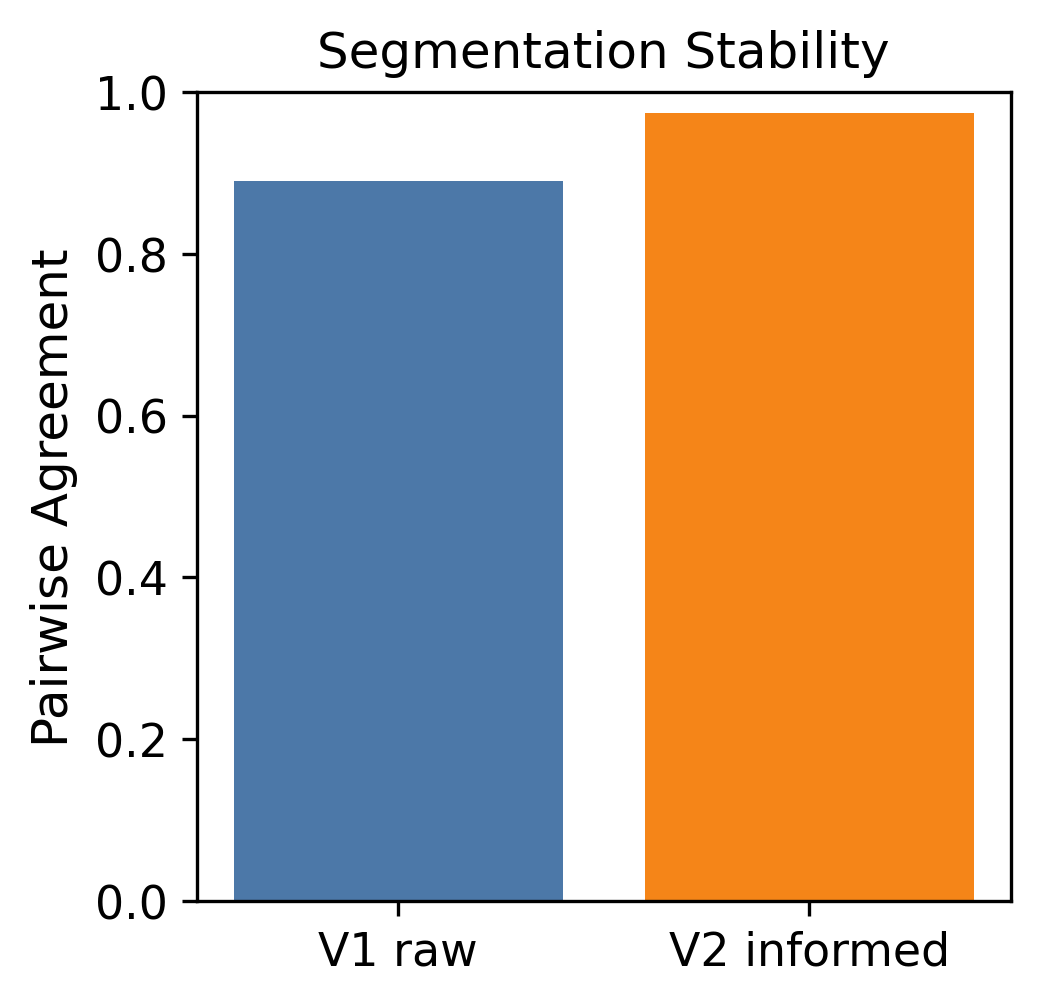
\includegraphics[width=\linewidth]{segmentation_stability_compare.png}
\caption{Stability comparison.}
\label{fig:stability}
\end{subfigure}
\caption{Model-selection evidence for the two segmentation variants.}
\label{fig:k-stability}
\end{figure}

Figure~\ref{fig:k-stability} and Table~\ref{tab:segment-variant-summary} show
the main pattern. Version 1 selects $k=5$ and achieves the better composite
score and silhouette, while Version 2 selects $k=8$ and achieves markedly higher
stability. This is a sensible outcome: adding the classifier score creates a
more repeatable structure, but it also pushes the space toward finer, more
score-driven premium splits.

I would report V1 as the primary segmentation in the take-home submission and
keep V2 as the activatable downstream variant. V1 gives the cleaner client
narrative because every segment can be explained directly from census-style
demographic and labor variables. V2 is more operationally detailed because it
uses the classifier score to separate the affluent tail into narrower premium
subsegments, but that also makes it more dependent on the quality and stability
of the supervised model. If the client wants a simple operating workflow, I
would deploy V1 only and not expose V2. If the activation team can support finer
premium subsegments, I would use V2 only downstream after the primary scoring
decision has already been made.

\begin{table}[!htbp]
\centering
\small
\caption{Segmentation pipeline comparison.}
\label{tab:segment-variant-summary}
\begin{tabular}{lcccc}
\toprule
Scheme & $k$ & Best Score & Silhouette & Stability \\
\midrule
V1 raw-feature unsupervised & 5 & 1.722 & 0.381 & 0.891 \\
V2 classifier-informed & 8 & 1.611 & 0.337 & 0.975 \\
\bottomrule
\end{tabular}
\end{table}

\subsection{How The Segment Structures Differ}

The next set of figures replaces text-only persona descriptions with auditable
evidence. Figure~\ref{fig:position-heat} shows the same V1 and V2 segments in a
common positioning chart and a common profile heatmap. Version 1 has one
small, college-leaning professional niche and one broader married full-year
working segment.
Version 2 preserves those low-income structural groups, but it splits the
high-income region into several more targeted segments. In other words, the
classifier-informed pipeline does not invent a new market structure from
nothing; it refines the affluent tail.

\begin{figure}[!htbp]
\centering
\begin{subfigure}[t]{0.48\linewidth}
\centering
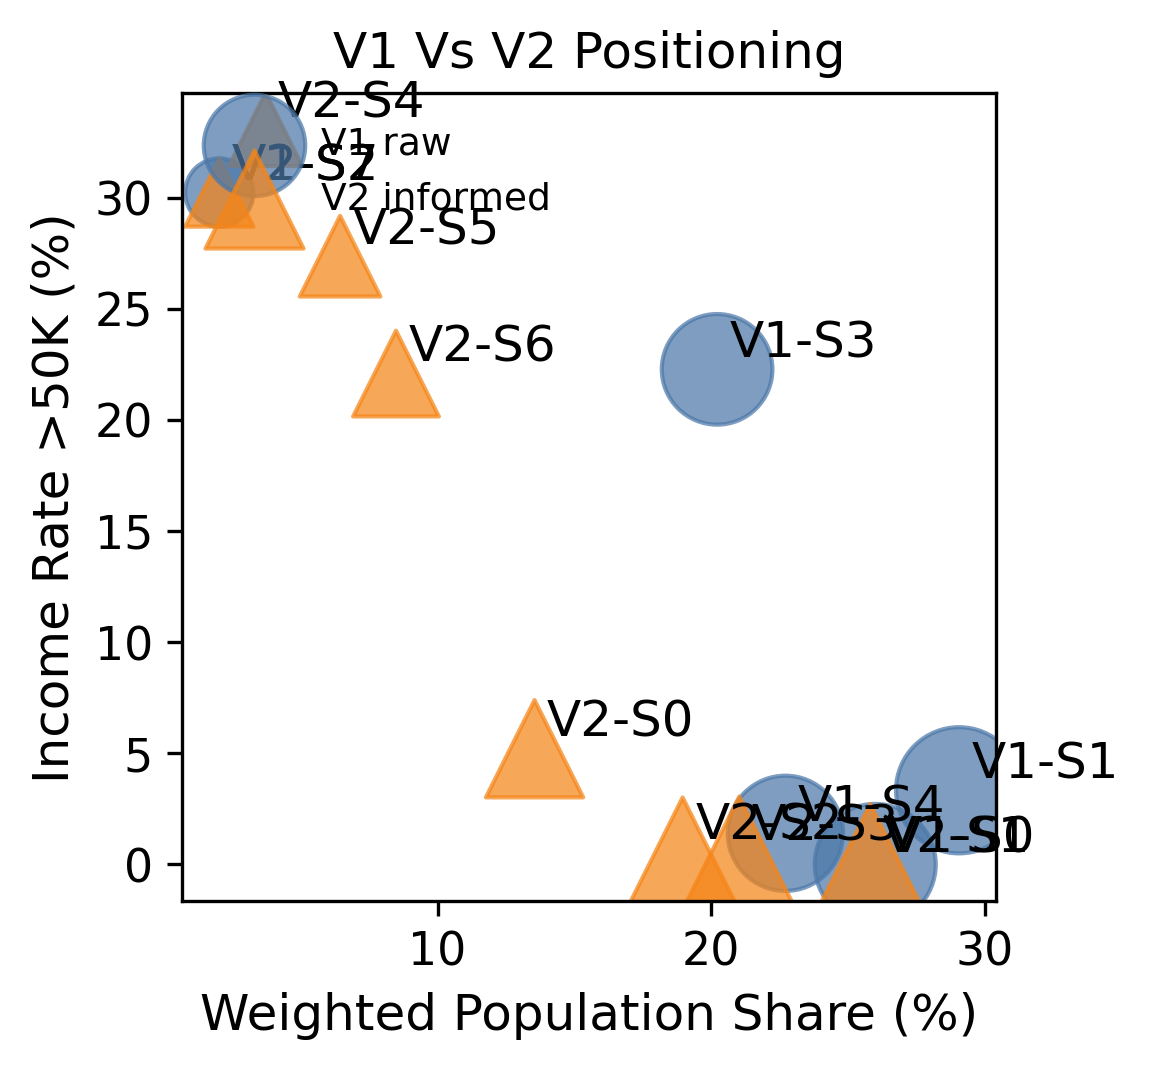
\includegraphics[width=\linewidth]{segmentation_positioning_compare.png}
\caption{Positioning of V1 and V2 segments.}
\label{fig:positioning}
\end{subfigure}
\hfill
\begin{subfigure}[t]{0.48\linewidth}
\centering
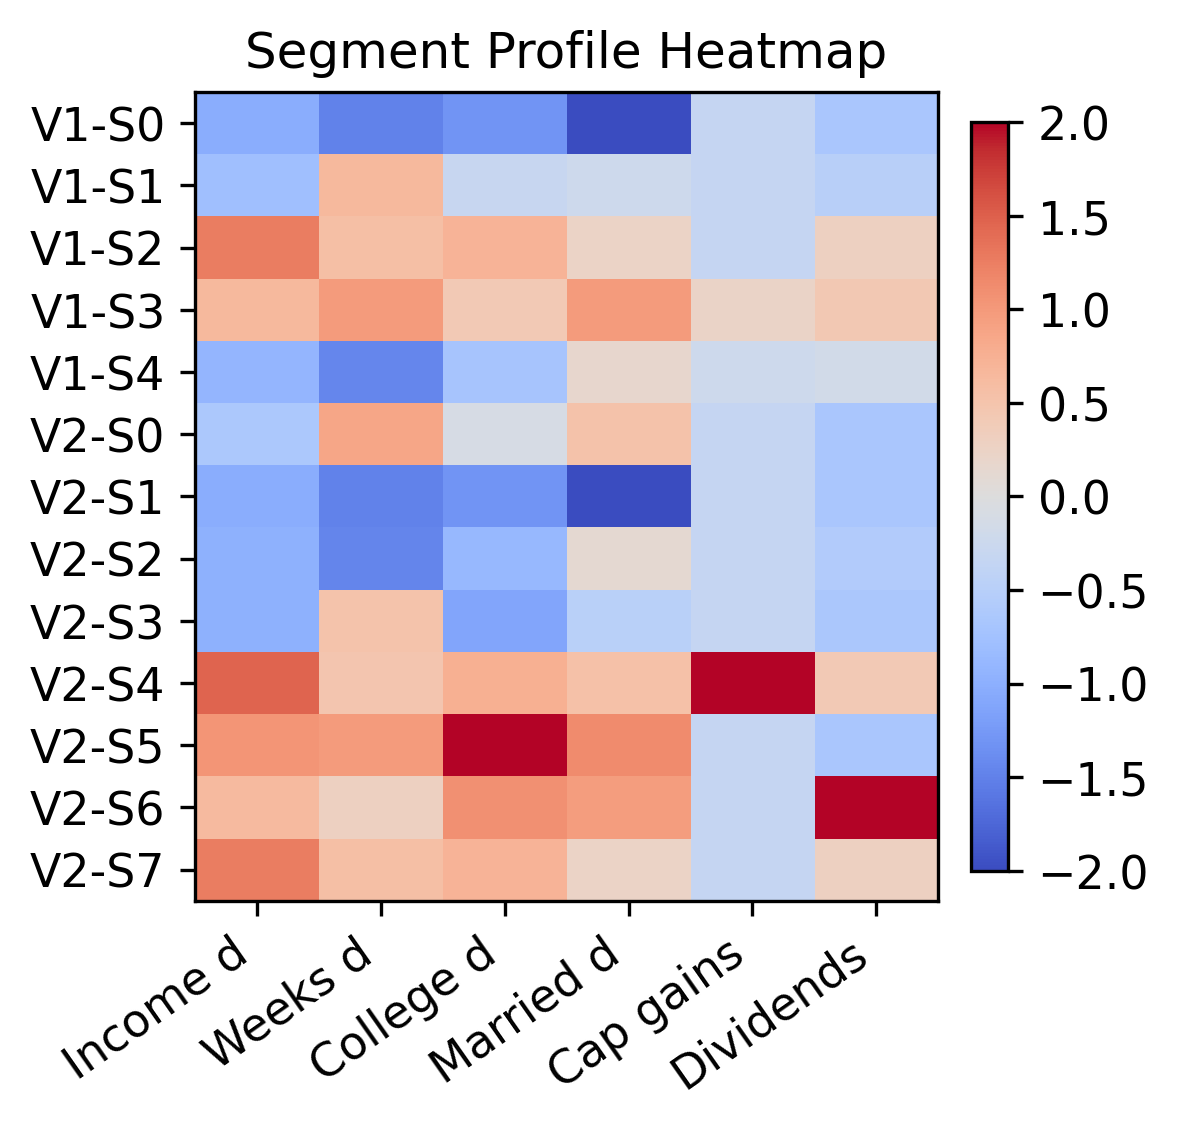
\includegraphics[width=\linewidth]{segmentation_profile_heatmap.png}
\caption{Joint standardized profile heatmap.}
\label{fig:heatmap}
\end{subfigure}
\caption{Direct comparison of V1 and classifier-informed V2 segment structure.}
\label{fig:position-heat}
\end{figure}

The heatmap is especially informative. The V1 high-value segments already have
positive deltas on income rate, weeks worked, college attainment, and marriage.
Version 2 then separates that high-value population into multiple subsegments
with different asset and education signatures, including one capital-gains-heavy
cluster and several college-dense mid-career clusters. That is why V2 is useful
as an advanced marketing overlay even though V1 remains the better main report
choice.

\begin{figure}[!htbp]
\centering
\begin{subfigure}[t]{0.48\linewidth}
\centering
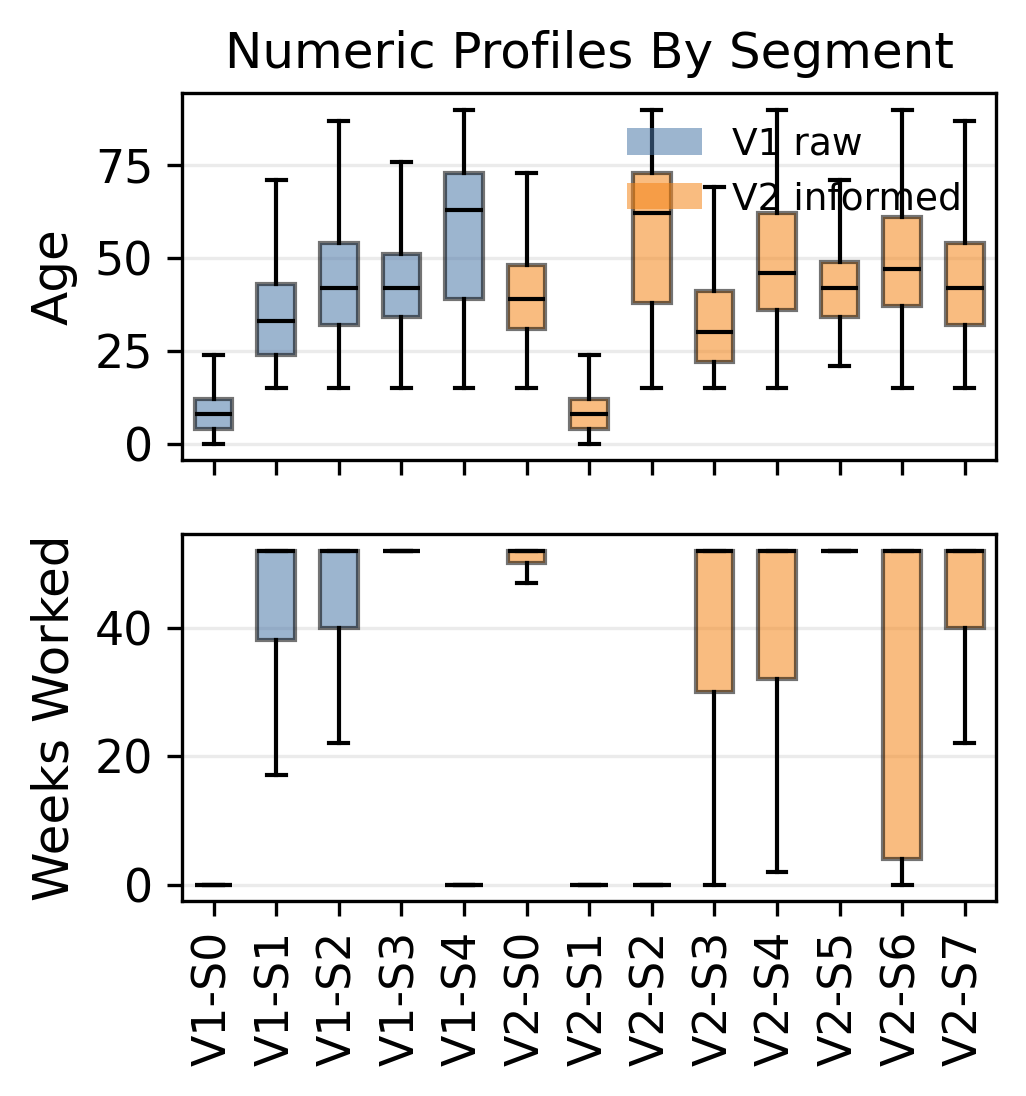
\includegraphics[width=\linewidth]{segmentation_numeric_boxplots.png}
\caption{Numeric differences by segment.}
\label{fig:num-box}
\end{subfigure}
\hfill
\begin{subfigure}[t]{0.48\linewidth}
\centering
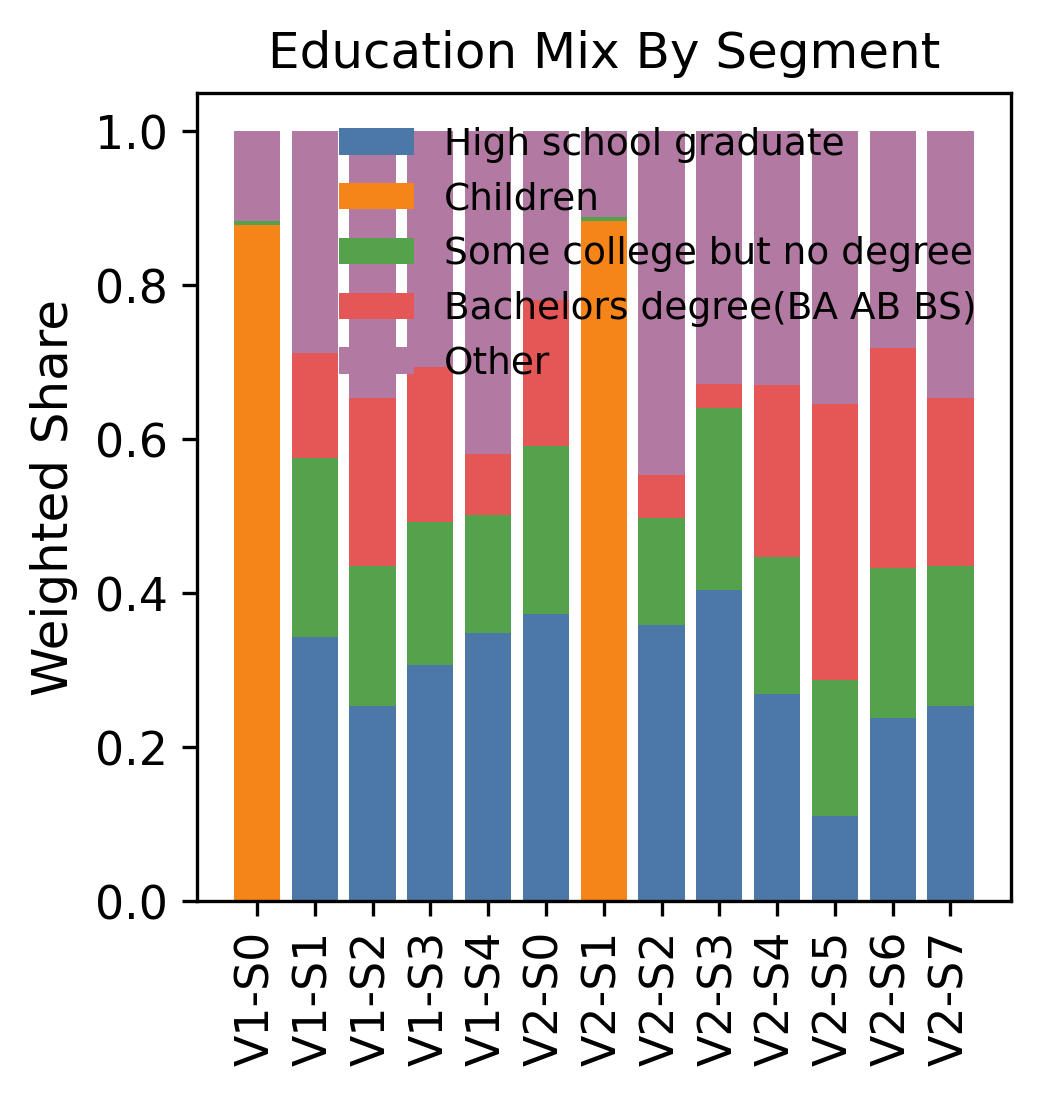
\includegraphics[width=\linewidth]{segmentation_education_composition.png}
\caption{Education mix by segment.}
\label{fig:edu-comp}
\end{subfigure}
\caption{Distributional and categorical evidence for segment distinctness.}
\label{fig:segment-audit}
\end{figure}

Figure~\ref{fig:segment-audit} provides more rigorous support for the personas.
The numeric boxplots show that age and labor intensity are not only different in
their means but also in their distributional spread. The education composition
chart shows that the classifier-informed high-income segments become more
Bachelor's-heavy and more differentiated than in Version 1, which is exactly the
kind of refinement expected when the clustering algorithm is allowed to use a
propensity score.

From a retail-marketing mechanics perspective, these differences affect product
tier, promotion aggressiveness, contact frequency, and expected ROI per
impression. Higher-income, college-dense, labor-attached segments justify
premium assortment, lower discount depth, and higher-touch channels because the
expected margin per contact is larger. Lower-propensity or structurally
non-working groups should receive lower-cost awareness messaging, softer
promotions, and lower contact frequency because repeated premium offers are more
likely to create waste than conversion. This is why the segmentation layer is
useful: it changes not only who gets contacted, but also what gets offered and
through which channel.

\subsection{Version 1 Personas For The Main Submission}

Even after adding the V2 comparison, Version 1 remains the best main-report
segmentation because it is easier to explain to a client without relying on a
supervised score. Table~\ref{tab:segment-personas} keeps the Version 1 persona
layer in a concise format.

\begin{table}[!htbp]
\centering
\small
\caption{Version 1 evidence A: segment personas and activation guidance.}
\label{tab:segment-personas}
\begin{tabularx}{\linewidth}{>{\raggedright\arraybackslash}p{1.0cm} >{\raggedright\arraybackslash}p{2.3cm} >{\raggedleft\arraybackslash}p{1.1cm} >{\raggedleft\arraybackslash}p{1.2cm} X}
\toprule
ID & Persona & Share & Income Rate & Suggested Action \\
\midrule
S0 & Youth / dependent households & 26.0\% & 0.0\% & De-prioritize premium targeting; use low-cost or family-oriented messaging. \\
S1 & Mainstream employed clerical households & 29.1\% & 3.3\% & Use value messaging, practical bundles, and moderate-contact campaigns. \\
S2 & College-leaning professional niche & 2.0\% & 30.2\% & Target with premium products, cross-sell, and high expected-value offers. \\
S3 & Married full-year upper-mid households & 20.2\% & 22.3\% & Position upper-mid-tier offers around reliability, family value, and productivity. \\
S4 & Older non-working households & 22.7\% & 1.4\% & Use low-frequency retention and age-appropriate service messaging. \\
\bottomrule
\end{tabularx}
\end{table}

\vspace{-2pt}
\begin{table}[!htbp]
\centering
\small
\caption{Version 1 evidence B: absolute profile summary.}
\label{tab:segment-profile-absolute}
\begin{tabular}{lcccccc}
\toprule
Seg & Share & Income & Weeks & College+ & Married & Cap gains+ \\
\midrule
S0 & 26.0\% & 0.0\% & 0.1 & 0.0\% & 0.0\% & 0.0\% \\
S1 & 29.1\% & 3.3\% & 43.0 & 18.4\% & 46.3\% & 0.0\% \\
S2 & 2.0\% & 30.2\% & 41.5 & 37.4\% & 57.9\% & 0.0\% \\
S3 & 20.2\% & 22.3\% & 49.4 & 32.0\% & 75.8\% & 15.0\% \\
S4 & 22.7\% & 1.4\% & 1.0 & 11.3\% & 55.9\% & 3.0\% \\
\bottomrule
\end{tabular}
\end{table}

The key business interpretation is straightforward. Segment S2 (professional
niche) is the smallest but highest-value niche for premium campaigns. Segment S3
(full-year upper-mid) is the scalable middle-to-upper tier audience. The
quantitative reason is clear in Table~\ref{tab:segment-profile-absolute}: S2 has
the highest rate-based efficiency at 30.2\% income incidence, but S3 carries
about 7.35x as much expected positive mass because its weighted share is much
larger while its income rate remains high at 22.3\%. Segments S0 and S4 should
not absorb premium budget. Segment S1 is a broad mainstream audience suited to
value-oriented but still personalized communication.

I recommend the following deployment priorities. If premium campaign budget is
limited, prioritize S2 first for margin efficiency and S3 second for scalable
upper-mid-tier conversion. If the goal is scale-maximizing expansion, use S3
first because it is materially larger while still retaining strong income
propensity. If the goal is low-cost awareness, S1 is the best broad audience and
S0/S4 should only be touched with inexpensive channels or family/lifecycle
relevant messaging. This trade-off is acceptable because the segment structure
cleanly separates expected value from audience size rather than forcing one
compromise segment to do both jobs.

\section{Final Recommendation}

The final recommended stack is:

\begin{itemize}
\item \textbf{Primary classifier:} LightGBM. It combines the best PR-AUC, best
weighted log loss, best operating F1 among the deployed models, and the best
calibration profile.
\item \textbf{Primary segmentation:} Version 1 raw-feature unsupervised
segmentation. It provides the cleanest methodological story and the strongest
balance of interpretability and cluster quality.
\item \textbf{Advanced segmentation overlay:} Version 2 classifier-informed
segmentation. It should be used when the client wants finer premium-audience
splits and is comfortable with a segmentation layer informed by the classifier
score.
\end{itemize}

The preferred deployment choice is to first rank the population with the
LightGBM score, then personalize campaign content and product tier using the
Version 1 segments. If a downstream activation team wants more refined
high-income subsegments, the Version 2 assignments can be used as a secondary
overlay.

I would not use classifier-only targeting as the entire operating policy, even
though the classifier is strong. The score is excellent for ranking propensity,
but it does not by itself decide product tier, promotion aggressiveness, channel
choice, or contact frequency. That independent value is exactly why segmentation
should remain in the workflow. I also would not launch V2 if the activation team
cannot operationalize finer premium subsegments, because in that setting the
extra complexity would add governance cost without enough incremental value.

In production I would deploy LightGBM first, expose V1 segmentation in the
client-facing workflow, and keep V2 behind the scenes as an advanced activation
option. I would monitor calibration drift, segment drift, and sparse-category
instability over time, because those are the most likely ways the current
decision logic could degrade after launch. I would also explicitly guard against
over-targeting premium offers to structurally low-propensity groups such as S0
and S4, because that failure mode creates budget waste while also weakening the
credibility of the targeting system.

\enlargethispage{2\baselineskip}
\section{References}

\begin{itemize}
\item LightGBM documentation: Microsoft LightGBM.
\item XGBoost documentation: XGBoost project documentation.
\item CatBoost documentation: Yandex CatBoost documentation.
\item FT-Transformer benchmark reference: Gorishniy et al., ``Revisiting Deep
Learning Models for Tabular Data,'' NeurIPS 2021.
\item Calibration reference: Niculescu-Mizil and Caruana, ``Predicting Good
Probabilities with Supervised Learning,'' ICML 2005.
\item Clustering metrics reference: scikit-learn documentation for silhouette,
Davies-Bouldin, and Calinski-Harabasz indices.
\end{itemize}

\section{Reproducibility Notes}

All report figures are generated directly from saved project artifacts by:

\begin{center}
\texttt{python plot/scripts/generate\_report\_figures.py}
\end{center}

The script writes all report figures into \texttt{plot/fig/}. The report source
file is \texttt{report.tex} at the repository root, on the same level as the
project \texttt{README.md}. If compiled with XeLaTeX or LuaLaTeX, the main font
is Times New Roman. If compiled with pdfLaTeX, the document falls back to a
portable Times-style package.

\end{document}
